\section{P-I-D analysis}\label{p-i-d-analysis}

This report introduces the effects of proportional, derivative and
integral gains, implemented by a conventional PID controller on a
Quanser's behaviour
\footnote{See Control Coursework Part 1 for a derivation of the transfer function used}.
This is assessed using time-domain and root locus results. A closed loop
PID controller, is used to reduce tracking error (\(e\)) between the
control input and the observed output \cite{ControlT54:online}. Through
correctly tuning the PID controller, it is desirable to achieve a sharp
response to user input.

\subsection{Proportional Feedback
Controller}\label{proportional-feedback-controller}

\begin{wrapfigure}{r}{0.5\textwidth}
\centering
\vspace{-35pt} % Space added to the top of the image
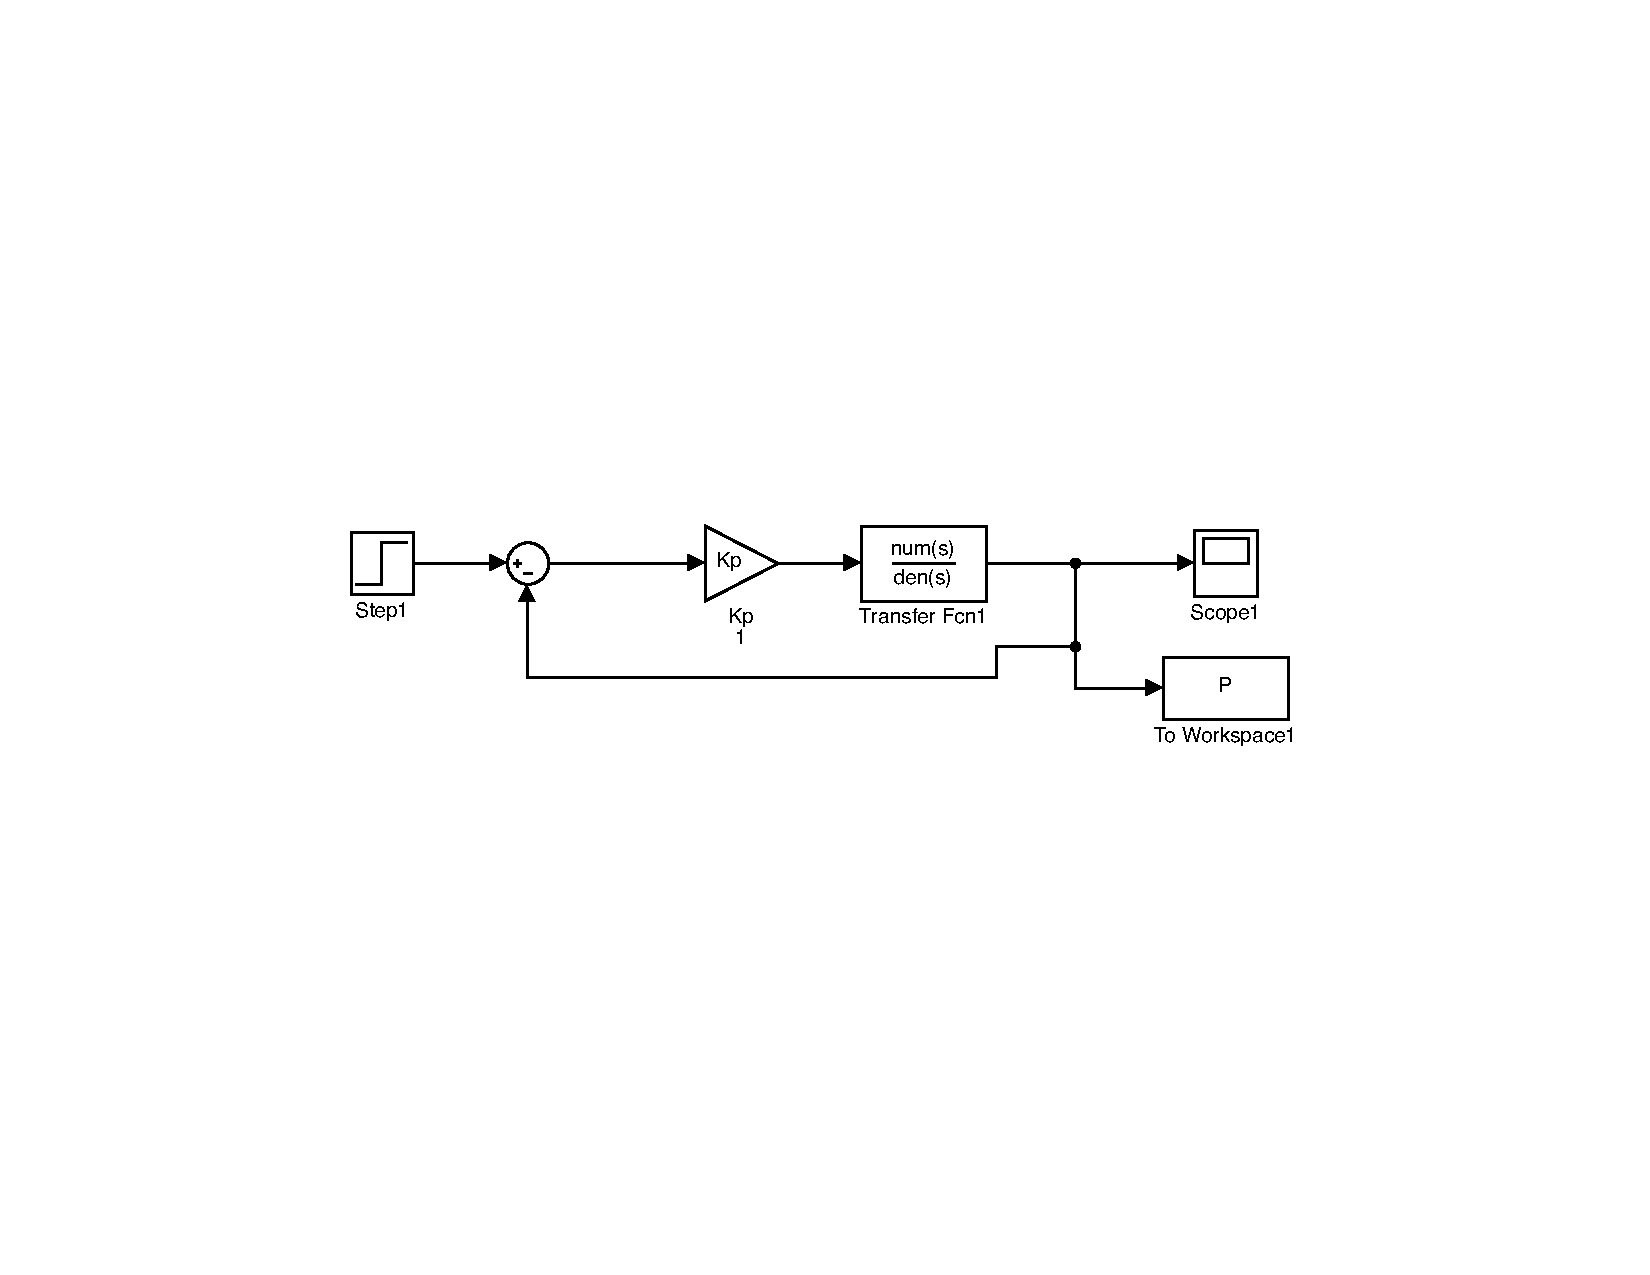
\includegraphics[trim = 0 0 0 0, clip, width=0.5\textwidth]{Psim.pdf}
\vspace{-25pt}
\caption{Proportional Feedback Controller}
\label{Psim}
\vspace{-15pt}
\end{wrapfigure}

Proportional gain control uses the \emph{Present} state of a plant to
error correct. The correction applied is proportional to the deviation
from the desired state of the plant. The result causes a highly
oscillatory system response, as the present error evaluates the
instantaneous state of the plant only. The simulation shown in Figure
\ref{Psim} found the effect of varying proportional gain (\(K_p\)) for
the Quanser transfer function. The simulation executed an iterative loop
with varying \(K_p\) from 0 to 0.1 in increments of 0.01. Figure
\ref{pres} shows the time domain response of increasing \(K_p\). When
\(K_p = 0\), a flat line was observed as there is no signal passing
through the plant. By extending proportional gain, the correction factor
became larger, increasing amplitude for higher \(K_p\) gains. The
\texttt{stepinfo()} function revealed that an increase in \(K_p\),
reduced both rise time and steady-state error while raising overshoot.

The root locus plot in \ref{pzp} allows observation of s-domain features
with varying proportional gain. For pure variation in proportional gain,
the (stable) poles are restricted to the same distance from the
imaginary axis. By increasing \(K_p\) the poles moved away from the real
axis in both directions, increasing natural-frequency (\(\omega_n\)) and
decreasing damping ratio \(\zeta\). The result verifies the observation
noted in the time domain response, as increased natural frequency will
lead to greater oscillatory behaviour, and reduced damping ratio
increases the overshoot.

\begin{figure}[H]
\centering
\begin{minipage}{.455\textwidth}
 \centering
 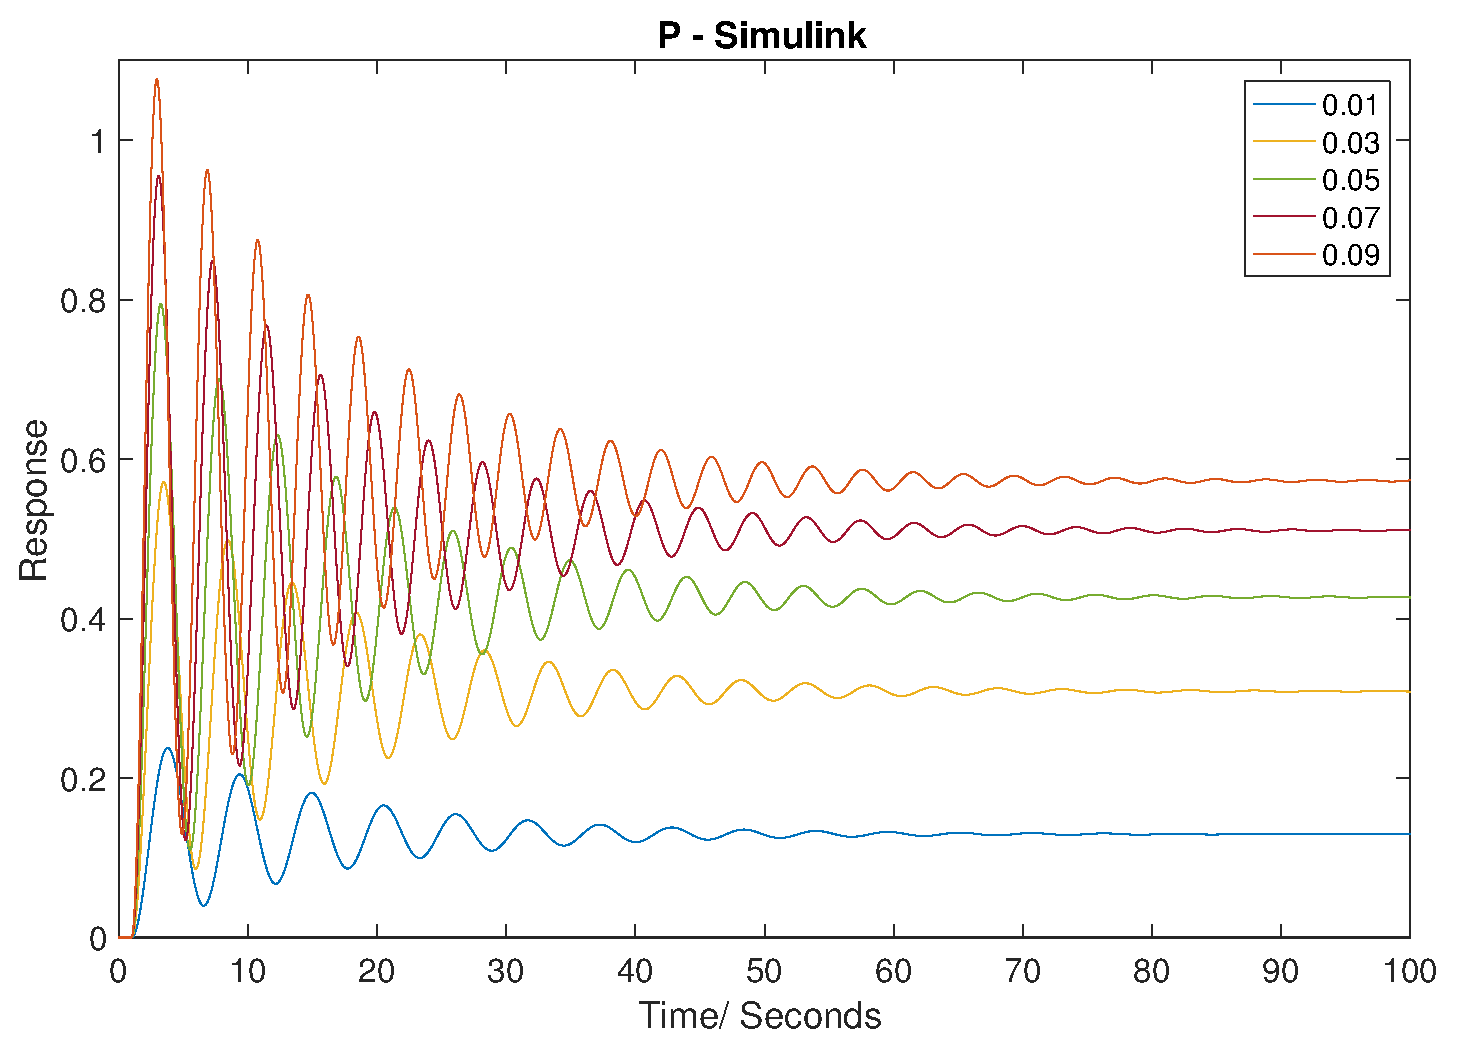
\includegraphics[trim = 0 0 0 0, clip, width=1\textwidth]{pres.eps}
 \caption{Response of Varying $K_p$}
 \label{pres}
\end{minipage}
\hfill
\begin{minipage}{.5\textwidth}
\centering
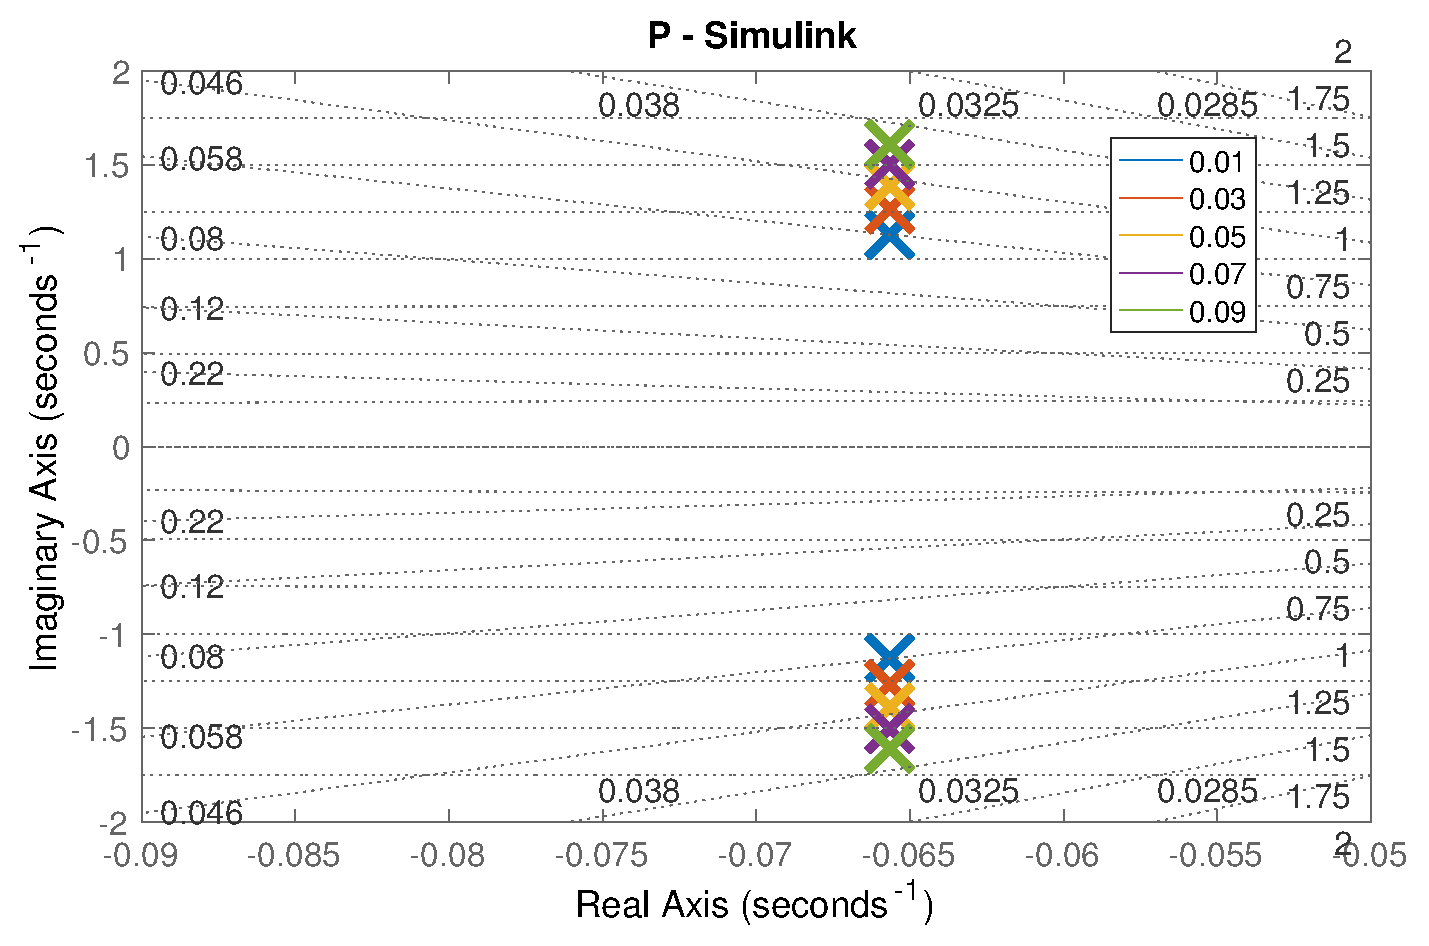
\includegraphics[trim = 0 0 0 0, clip, width=1\textwidth]{pzp.eps}
\caption{Poles of Varying $K_p$}
\label{pzp}
\end{minipage}
\vspace{-20pt}
\end{figure}

\subsection{Derivative Feedback
Controller}\label{derivative-feedback-controller}

\begin{wrapfigure}{r}{0.5\textwidth}
\centering
\vspace{-35pt} % Space added to the top of the image
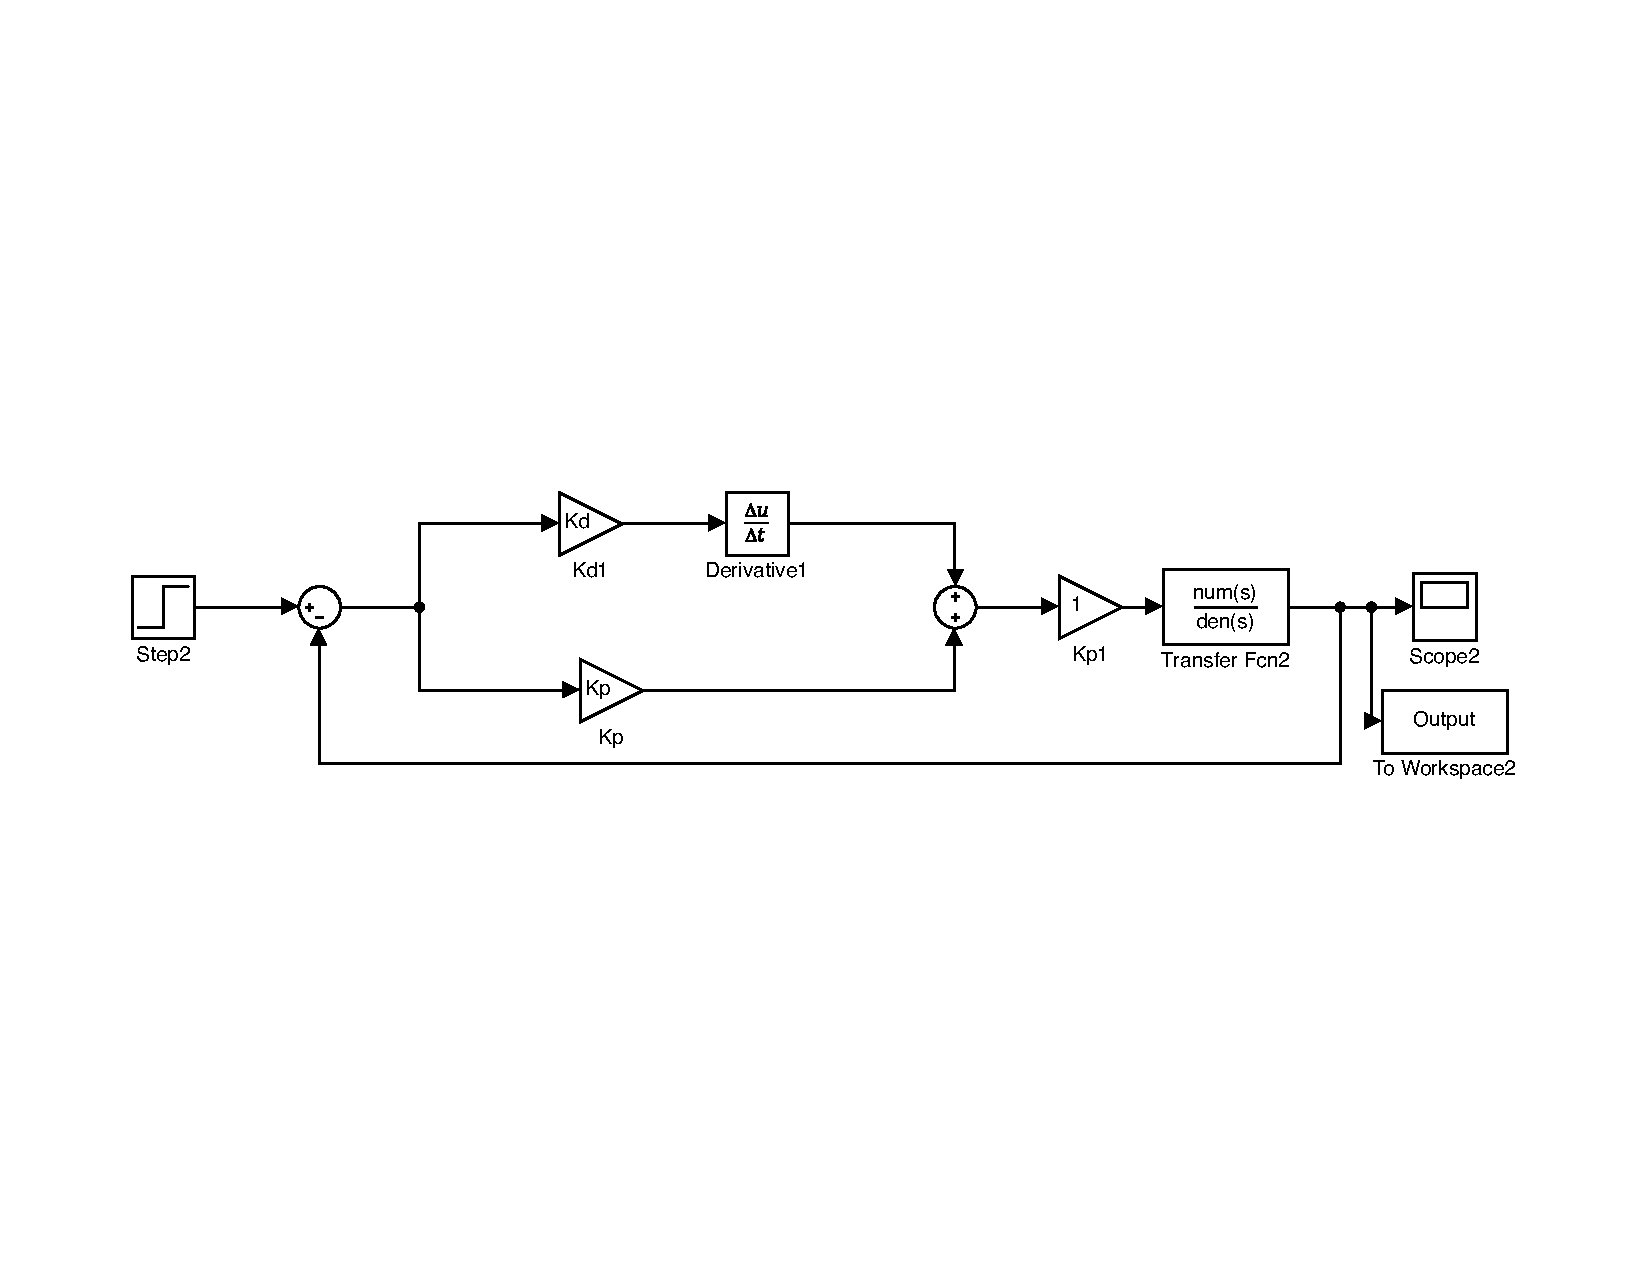
\includegraphics[trim = 0 0 0 0, clip, width=0.5\textwidth]{pd2.pdf}
\vspace{-10pt}
\caption{PD Feedback Controller}
\label{pd2}
\vspace{-25pt}
\end{wrapfigure}

Derivative control utilises the expected \emph{Future} state of the
system to pre-emptively correct the error signal, \(e\). This correction
is proportional to the rate of change of the system state at a point in
time. The system calculates the state of the plant in the future based
on the rate of change conditions and accounting for the effects in the
response. For this reason, a large damping effect is expected for
increasing derivative gain (\(K_d\)). The simulation in Figure \ref{pd2}
was implemented to observe the effect of purely varying derivative gain
with constant proportional gain, and the effect of varying both gains by
the same amount; controlled using the additional gain block after the
controller. Gain values in Figure \ref{vkpvkd} and Figure \ref{ckpvkd}
were incremented from 0 to 1 in increments of 0.1.

\begin{wrapfigure}{r}{0.45\textwidth}
\centering
\vspace{-15pt} % Space added to the top of the image
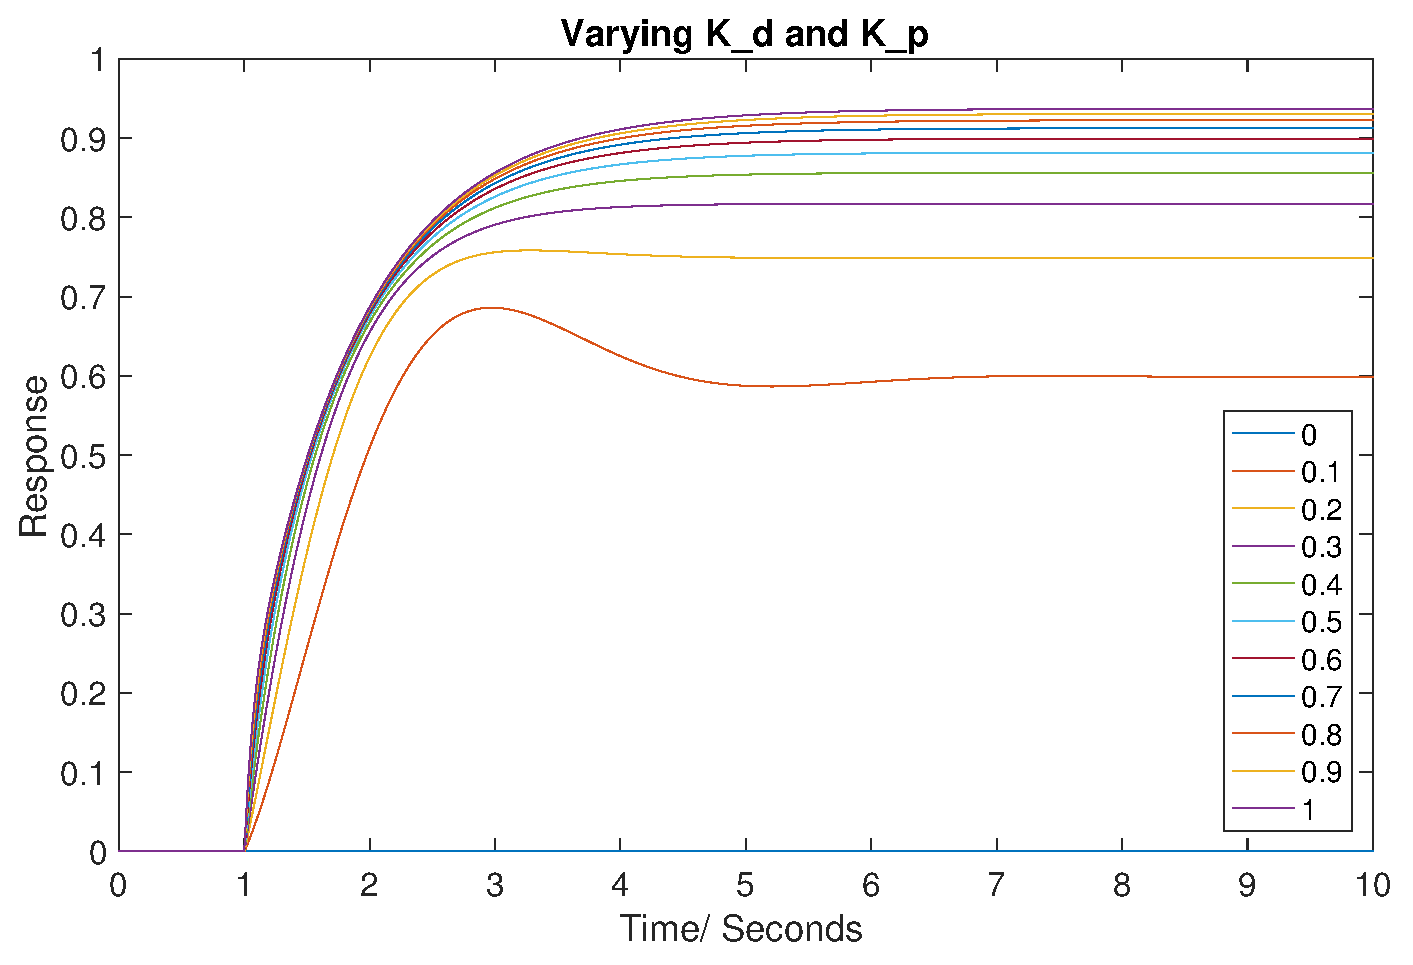
\includegraphics[trim = 0 0 0 0, clip, width=0.45\textwidth]{vkpvkd.eps}
\vspace{-10pt}
\caption{Time-Domain Response For Varying $K_p$ and Varying $K_d$}
\label{vkpvkd}
\vspace{-15pt}
\end{wrapfigure}

Both time domain responses show that increasing \(K_d\) has a greater
damping effect on oscillations, reducing overshoot while increasing rise
time. For a \(K_d = 0\), large oscillations were observed, decreasing
with higher gain values. For gain values 0.6 and above, both high
damping and quick settling times were observed. Increasing both \(K_d\)
and \(K_p\) by the same amount shows a reduction in rise time, overshoot
and steady-state error. The root locus S-domain metrics in Figure
\ref{pzd} show that as \(K_d\) increases the poles are shifted
negatively in the real axis. The semi-circular shape represents the line
of equal proportional gain, and the points represent varying \(K_d\) at
that \(K_p\) level. As \(K_d\) is increased, the polar angle also
increases. This implies poles closer to the real axis, (higher \(K_d\))
correspond to poles with greater damping; the natural frequency is
therefore reduced decreasing oscillatory behaviour.

\begin{figure}[H]
\centering
\begin{minipage}{.455\textwidth}
 \centering
 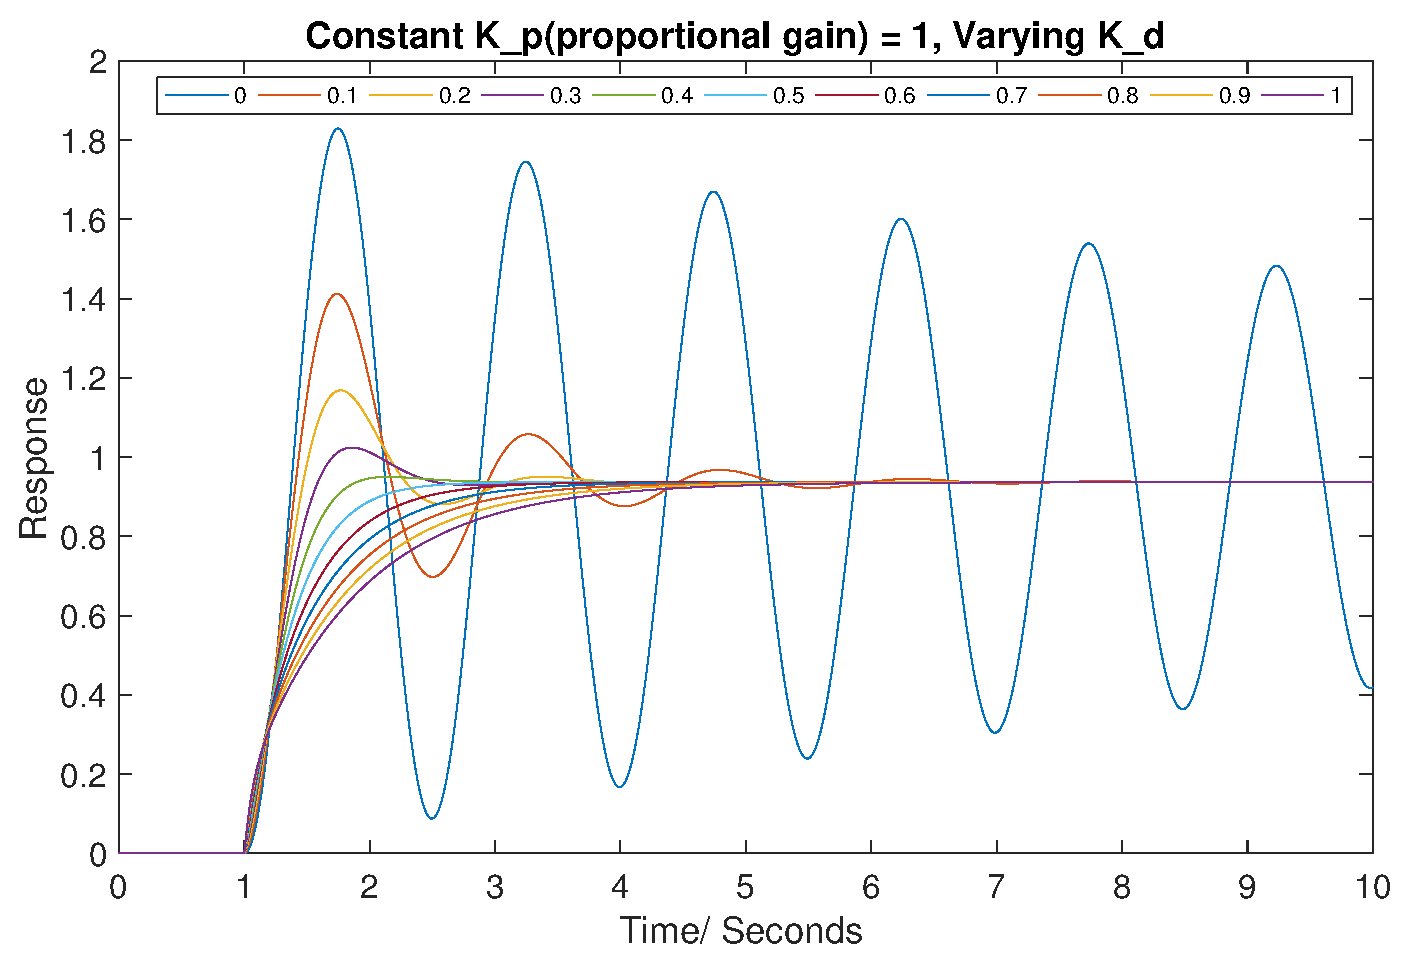
\includegraphics[trim = 0 0 0 0, clip, width=1\textwidth]{ckpvkd.eps}
 \caption{Time-Domain Response For Constant $K_p$ and Varying $K_d$}
 \label{ckpvkd}
\end{minipage}
\hfill
\begin{minipage}{.455\textwidth}
\centering
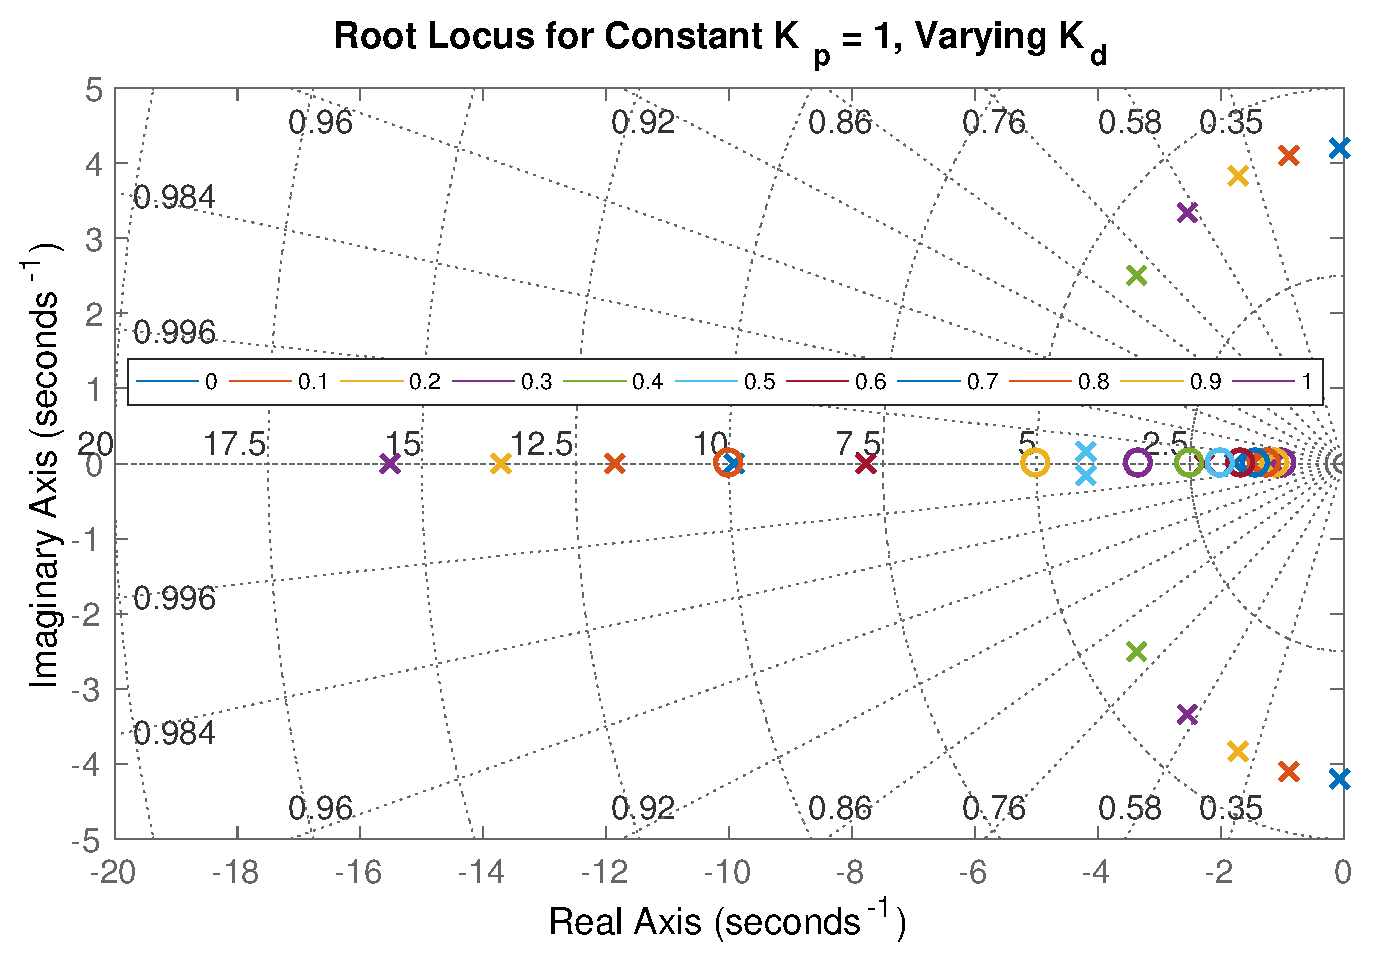
\includegraphics[trim = 0 0 0 0, clip, width=1\textwidth]{pzd.eps}
\caption{Poles of Constant $K_p$ and Varying $K_d$}
\label{pzd}
\end{minipage}
\vspace{-20pt}
\end{figure}

\subsection{Integral Action}\label{integral-action}

\begin{wrapfigure}{r}{0.5\textwidth}
\centering
\vspace{-15pt} % Space added to the top of the image
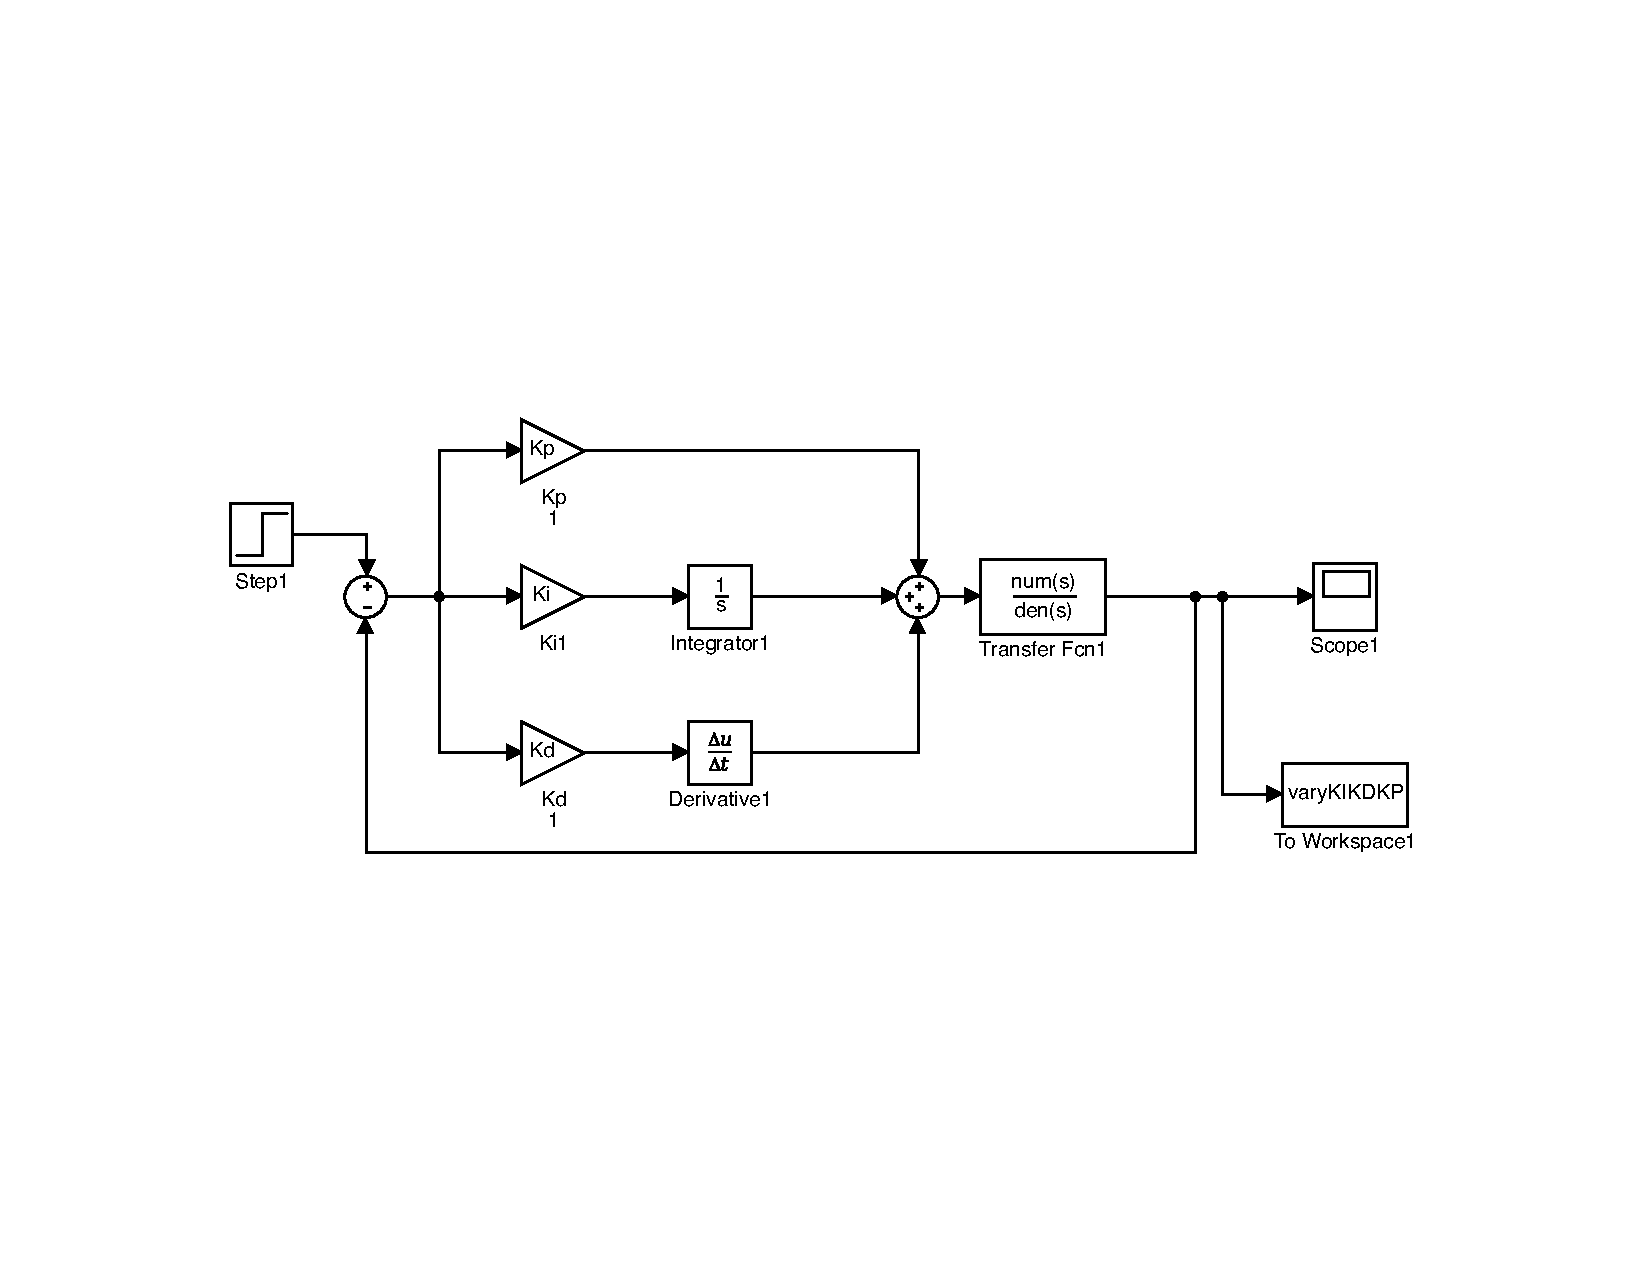
\includegraphics[trim = 0 0 0 0, clip, width=0.5\textwidth]{PIDp2.pdf}
\vspace{-10pt}
\caption{PID Feedback Controller}
\label{PIDp2}
\vspace{-15pt}
\end{wrapfigure}

Integral control utilises the \emph{Past} state of the system to produce
an error-correcting signal. The integral controller sums the historical
tracking error up to current time state, eliminating offset and leading
to zero steady state error. The simulation of a full PID controller is
shown in Figure \ref{PIDp2}. Figure \ref{ckpckdvki} shows the variation
of pure \(K_i\) with constant \(K_p\) and \(K_d\). Figure
\ref{vkpvkdvki} shows the variation of all three gains \(K_d\), \(K_i\)
and \(K_p\) by the same magnitude. This was implemented using a
gain-scaling block after the controller. The time domain plots confirm
the zero steady state error as the oscillations level to desired
response level.

\begin{figure}[h]
\centering
\begin{minipage}{.455\textwidth}
 \centering
 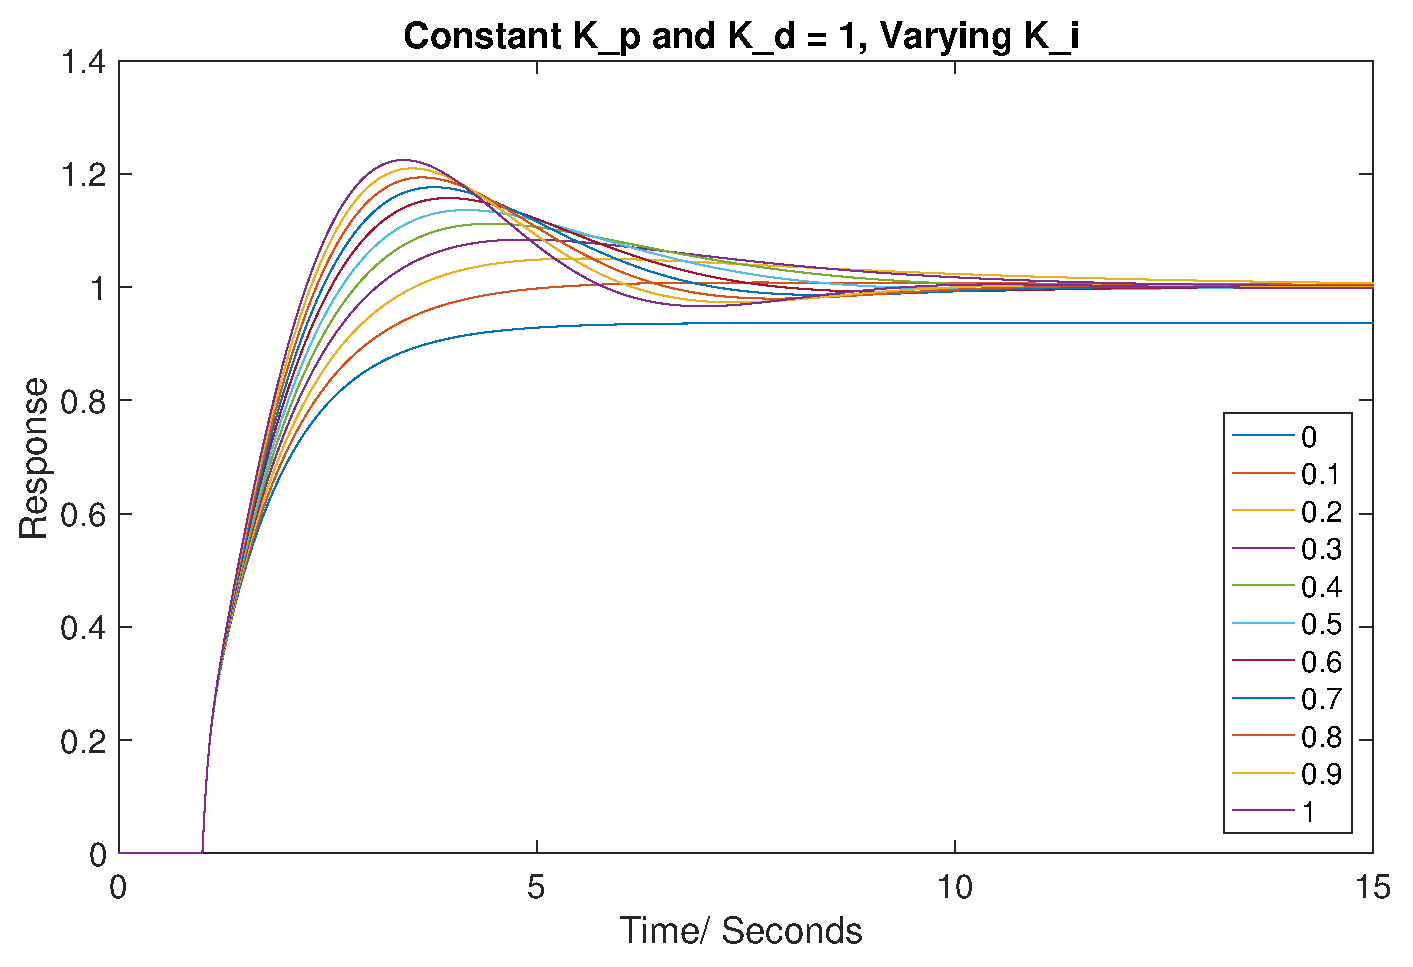
\includegraphics[trim = 0 0 0 0, clip, width=1\textwidth]{ckpckdvki.eps}
 \caption{Time-Domain Response For Constant $K_p$, $K_d$ and Varying $K_i$}
 \label{ckpckdvki}
\end{minipage}
\hfill
\begin{minipage}{.455\textwidth}
\centering
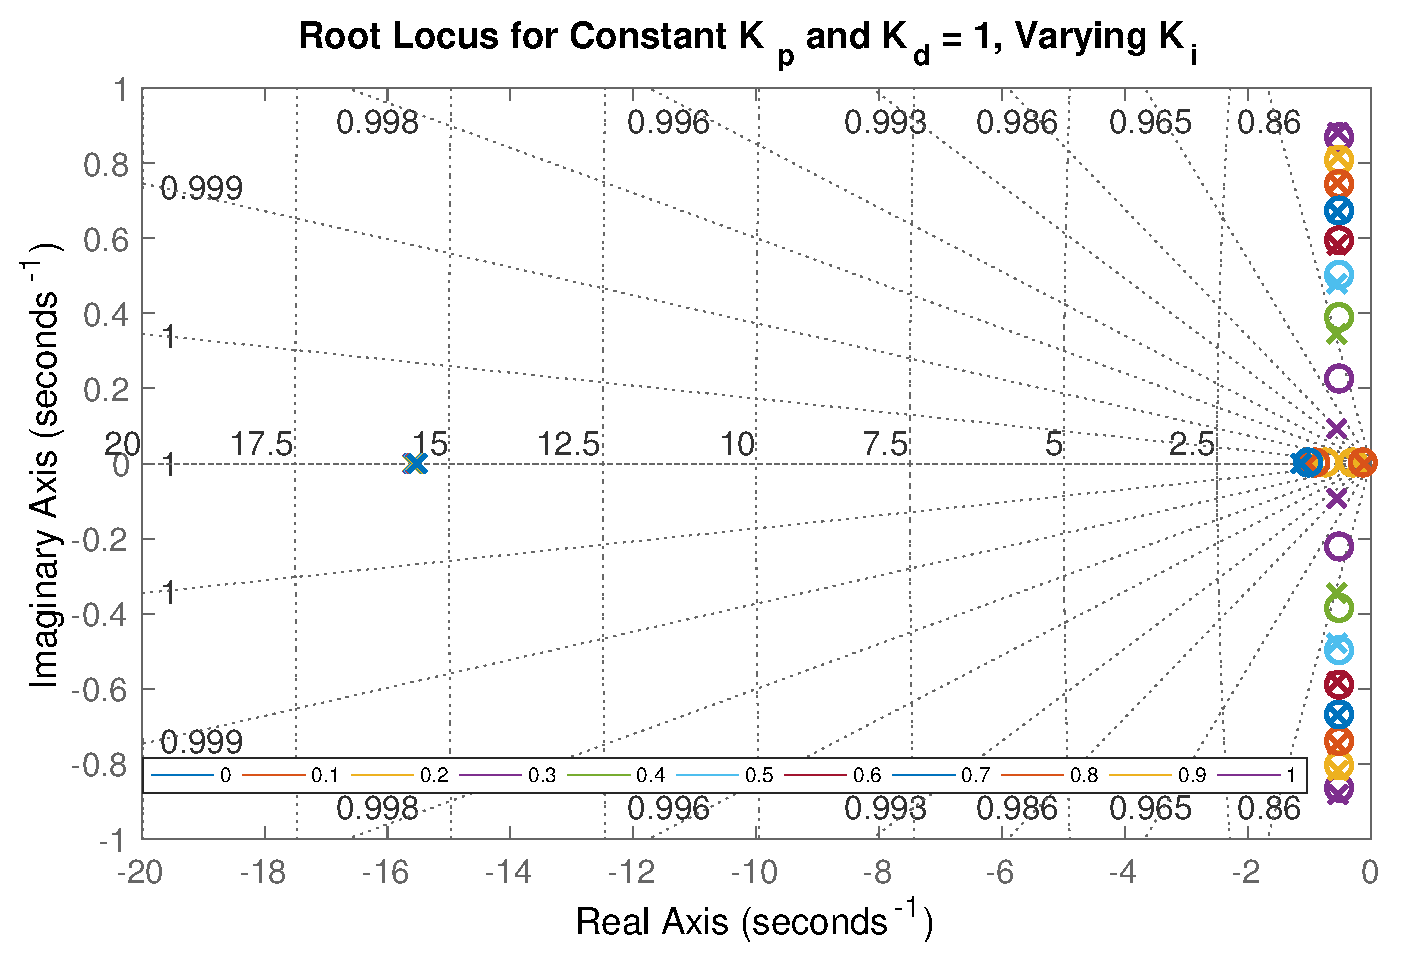
\includegraphics[trim = 0 0 0 0, clip, width=1\textwidth]{pzi.eps}
\caption{Poles of Constant $K_p$, $K_d$ and Varying $K_i$}
\label{pzi}
\end{minipage}
\vspace{-20pt}
\end{figure}

\begin{wrapfigure}{r}{0.5\textwidth}
\centering
\vspace{-5pt} % Space added to the top of the image
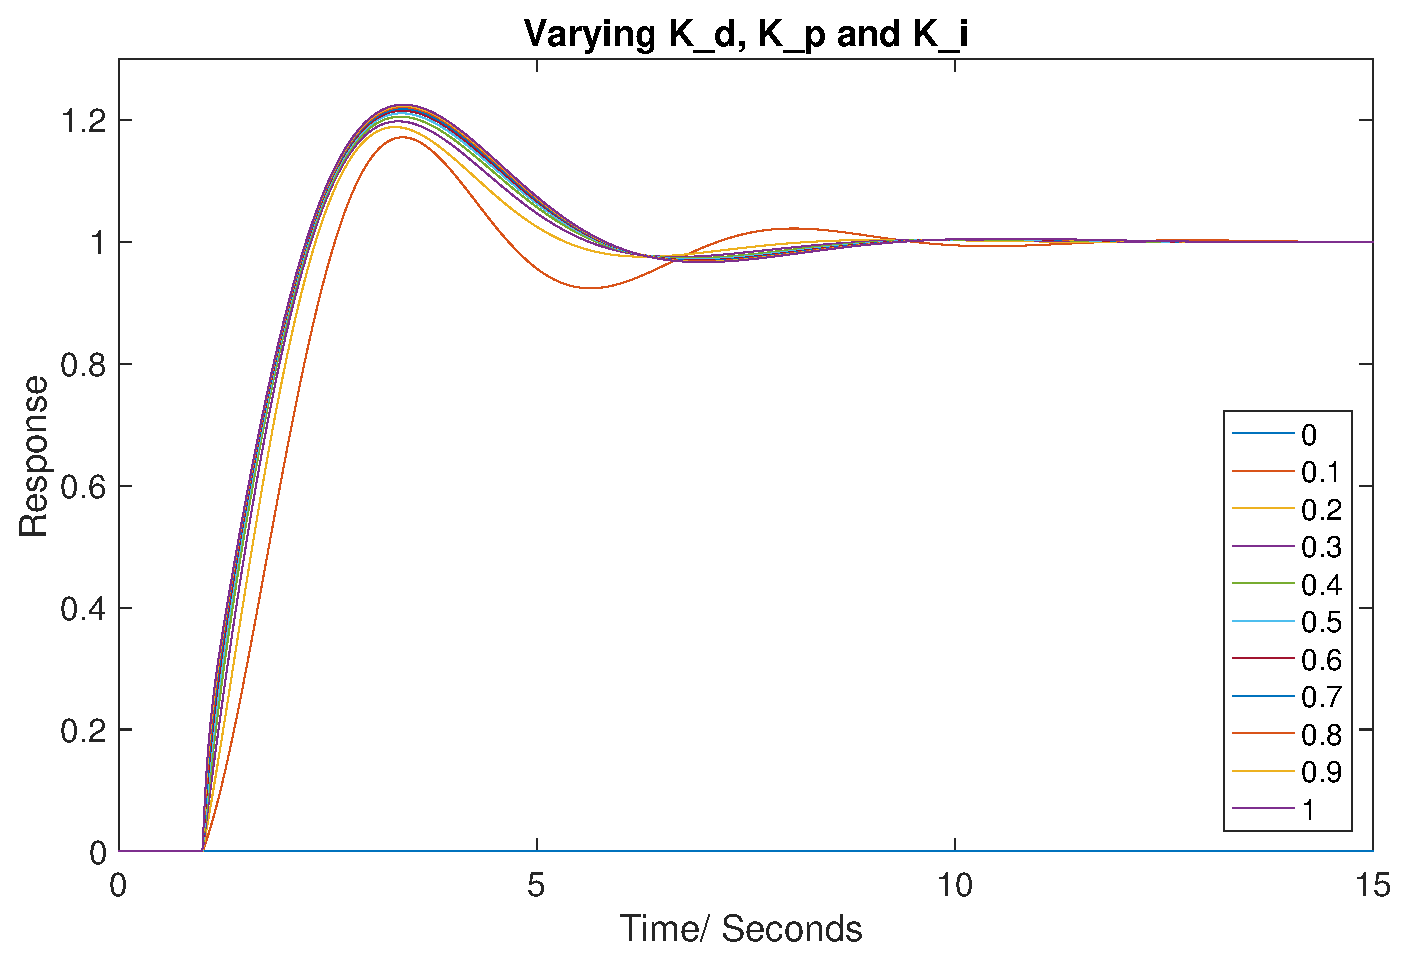
\includegraphics[trim = 0 0 0 0, clip, width=0.5\textwidth]{vkpvkdvki.eps}
\vspace{-10pt}
\caption{Time-Domain Response For Varying $K_p$, $K_d$ and $K_i$}
  \label{vkpvkdvki}
\vspace{-35pt}
\end{wrapfigure}

At \(K_i = 0\) there is steady state error that exists in the system,
but as integral gain increases the steady state error is eliminated.

\section{PID Design to Achieve Control
Requirements}\label{pid-design-to-achieve-control-requirements}

Through implementing the learning gained in part 1, a closed
loop-feedback controller was then developed for the theoretical Quanser
transfer function. This controller was tuned, through creating a script
which outputted the step response of the controller into a table using
the \texttt{stepinfo()}. Due to the steady state error response observed
through using either a P or PD controller, it was decided to iterate
different gains for a full PID, to obtain the optimum response.
Initially all gains were iterated using the gain-scaling block
(discussed in section \ref{integral-action}). Through observing the
different response, a rough estimate was found for all three gains,
which could then be individually tweaked based on the parameters shown
in Table \ref{paramtab}.The first order transfer function obtained in
Control part 1, was corrected using a more appropriate method for
calculation of \(\tau\). \(\tau = \zeta \times \omega_n\)

\subsection{Open Loop Transfer Function PID
Controller}\label{open-loop-transfer-function-pid-controller}

\begin{wraptable}{l}{0.5\textwidth}
\vspace{-10pt}
\caption{Effect of Gains on Objectives}
\vspace{-5pt}
\centering
 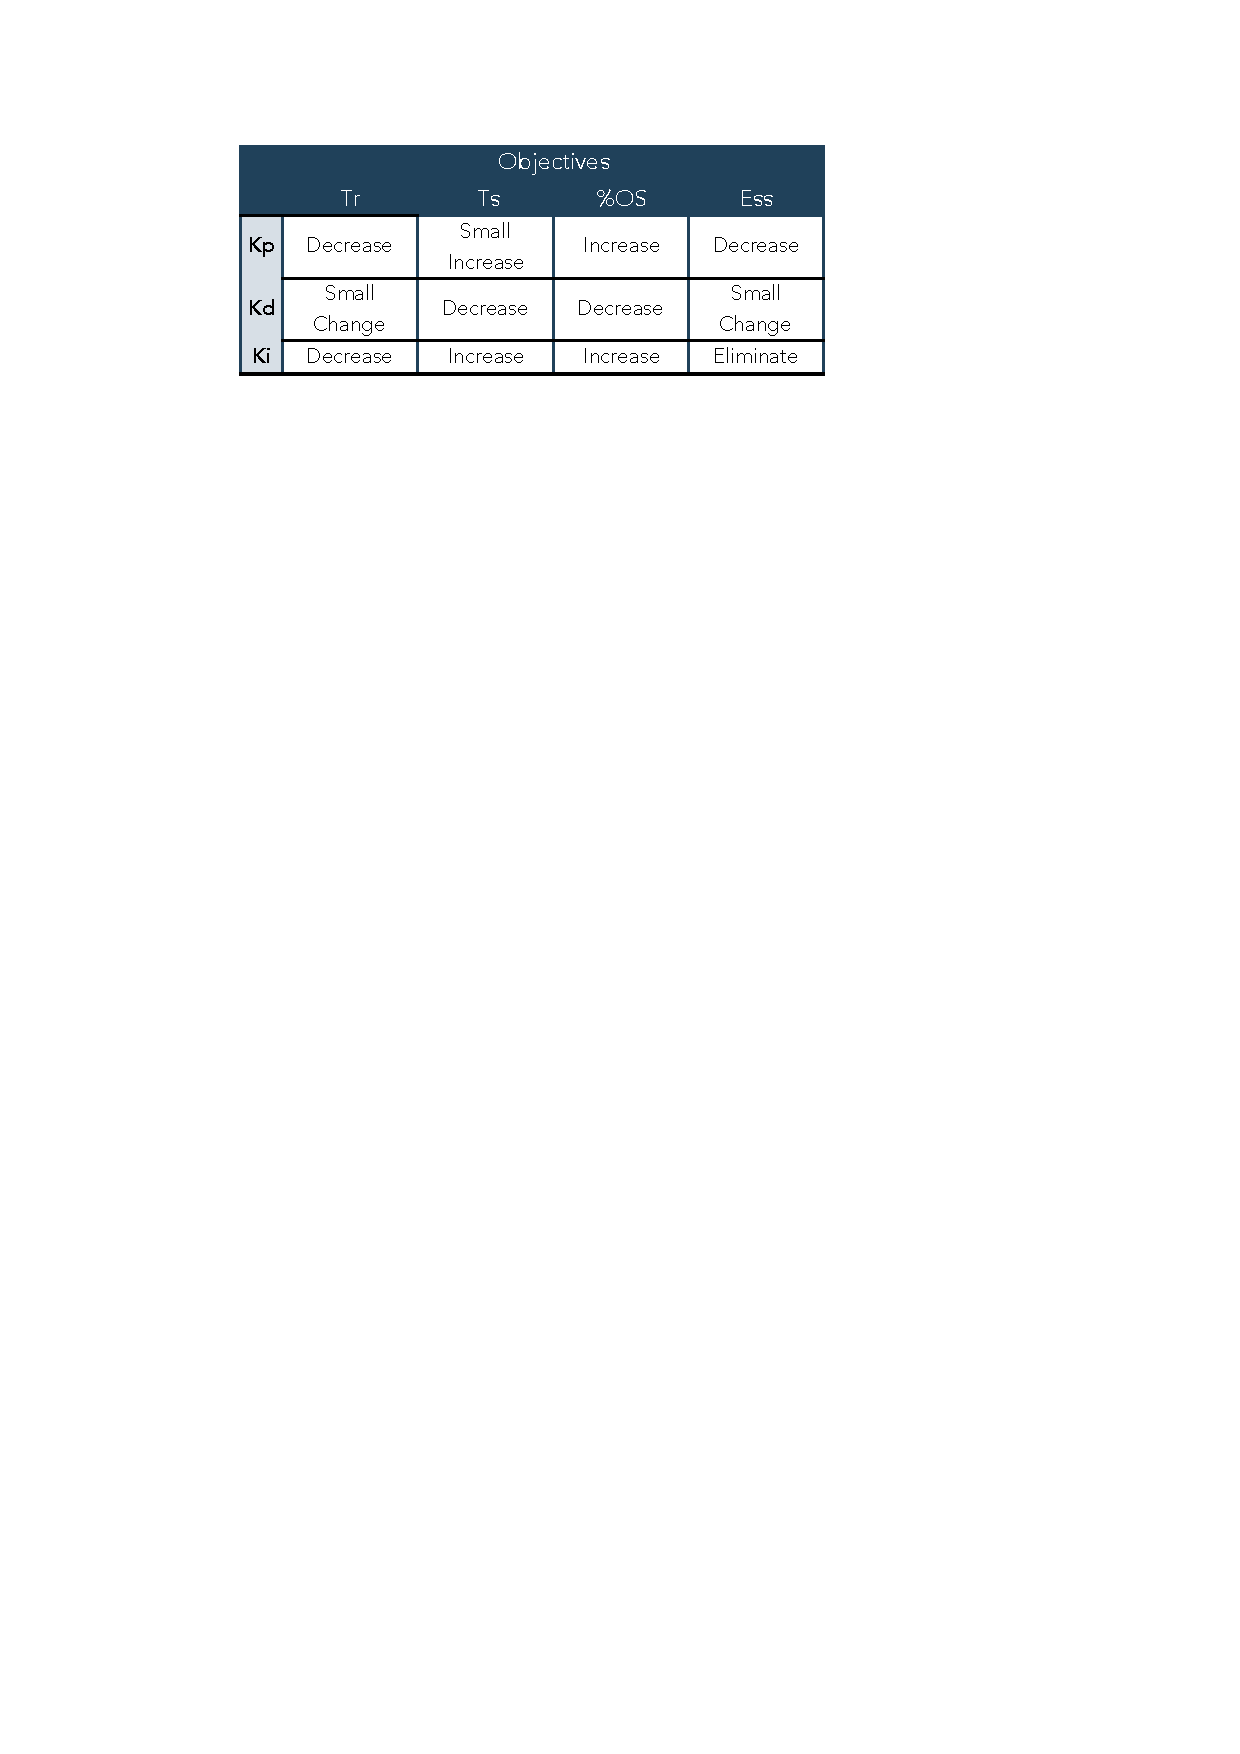
\includegraphics[trim = 0 0 0 0, clip, width=0.49\textwidth]{tableobj.pdf}
 \vspace{-15pt}
 \label{paramtab}
\end{wraptable}

As the proportional, integral and derivative gain values were adjusted
to tune the PID, the characteristics for changing each gain were
considered with reference to Table \ref{paramtab} . The controller was
then tuned as necessary to best meet the requirements .Testing several
PD controller structures, the resulting response showed poor steady
state error. It was found that a PID controller with stated gain values
produced optimal time domain metrics, which improved upon the provided
specifications.

\begin{figure}[H]
\centering
\begin{minipage}{.55\textwidth}
 \centering
 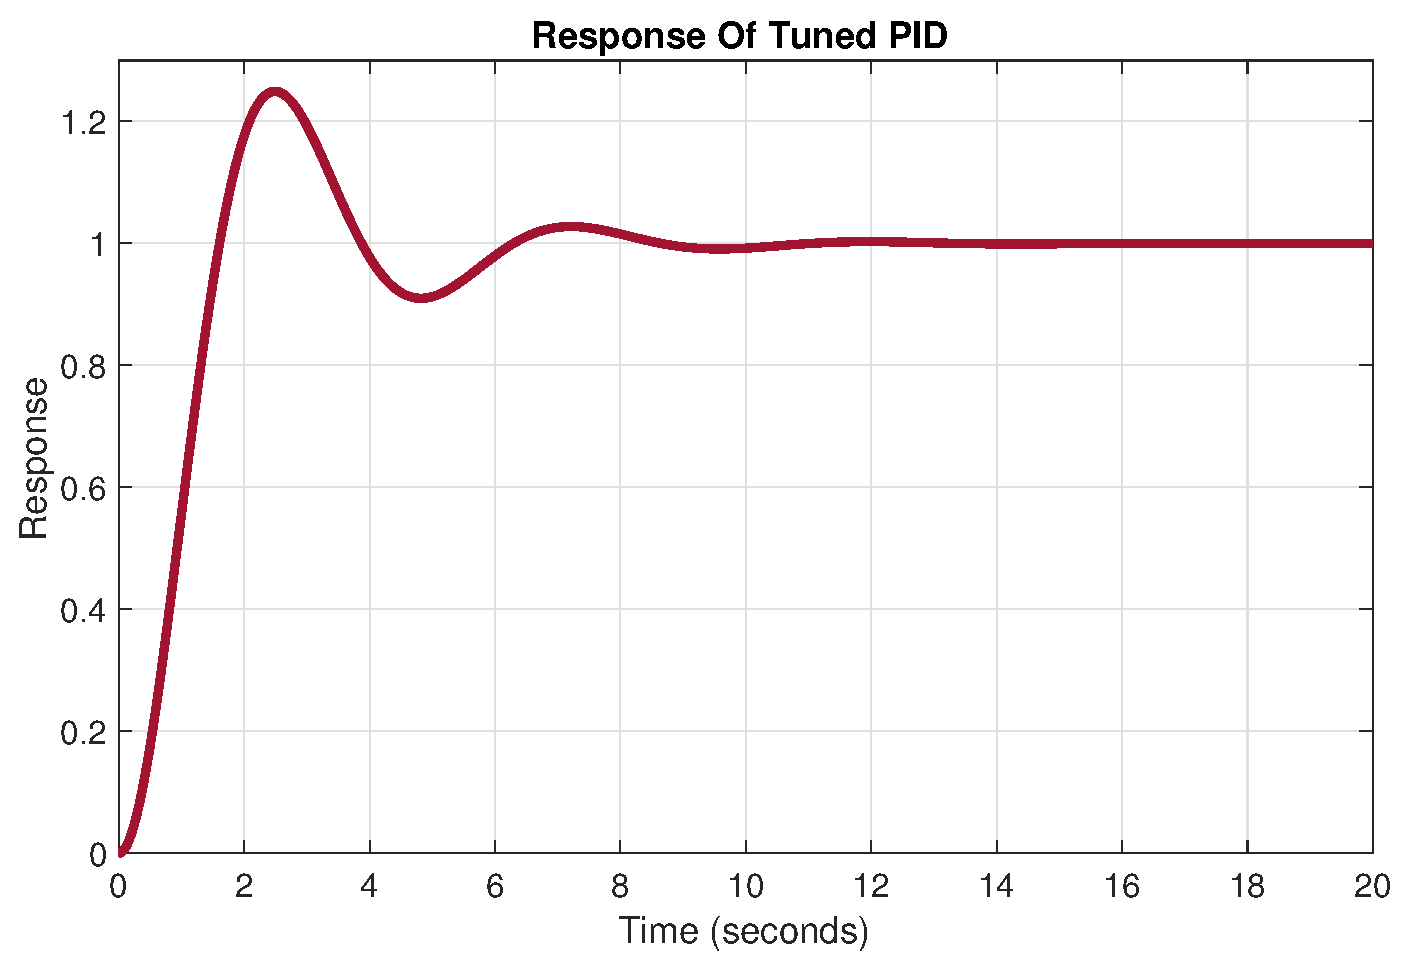
\includegraphics[trim = 0 0 0 0, clip, width=1\textwidth]{p2atun.eps}
 \vspace{-20pt}
 \caption{Tuned PID Response}
 \label{p2bres}
\end{minipage}
\hfill
\begin{minipage}{.35\textwidth}
\centering
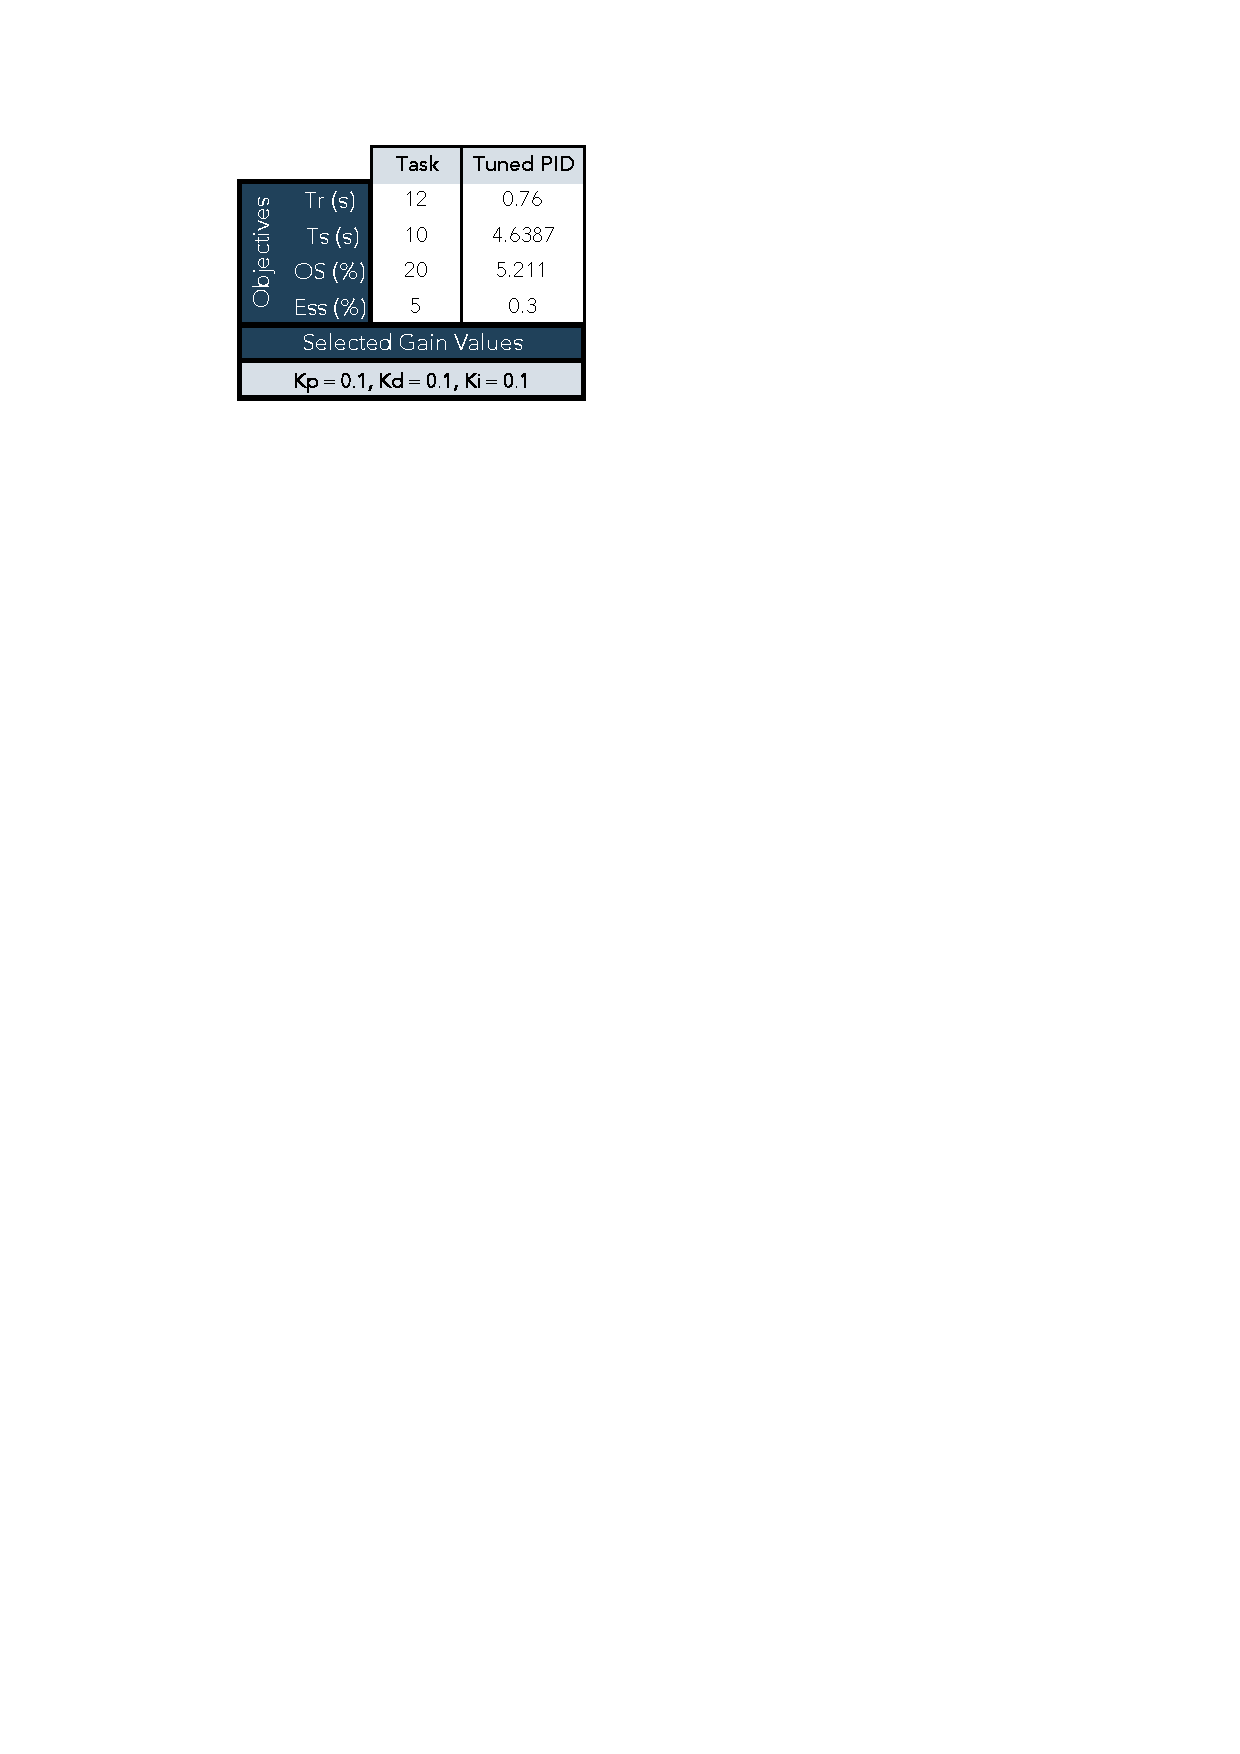
\includegraphics[trim = 0 0 0 0, clip, width=1\textwidth]{paramtuned.pdf}
\vspace{-10pt}
\caption{Tuned PID Transfer Function Values}
\label{paramtab}
\end{minipage}
\vspace{-20pt}
\end{figure}

\subsection{Tuned Quanser Controller}\label{tuned-quanser-controller}

A PID controller with the stated proportional, integral and derivative
gain values was created inside the SSC17\_QuanserPart2\_PIDdesign.slx
`controller block. The transfer function identified previously was input
into the empty `PLANT' block. This allowed observation of the expected
Quanser response for the chosen PID and plant configuration. In addition
the two other `extreme' plants were also tested to ensure the controller
was working effectively. The extreme plants were also used as a
procedure for modifying our Controller structure.

\begin{figure}[H]
\centering
\begin{minipage}{.495\textwidth}
 \centering
 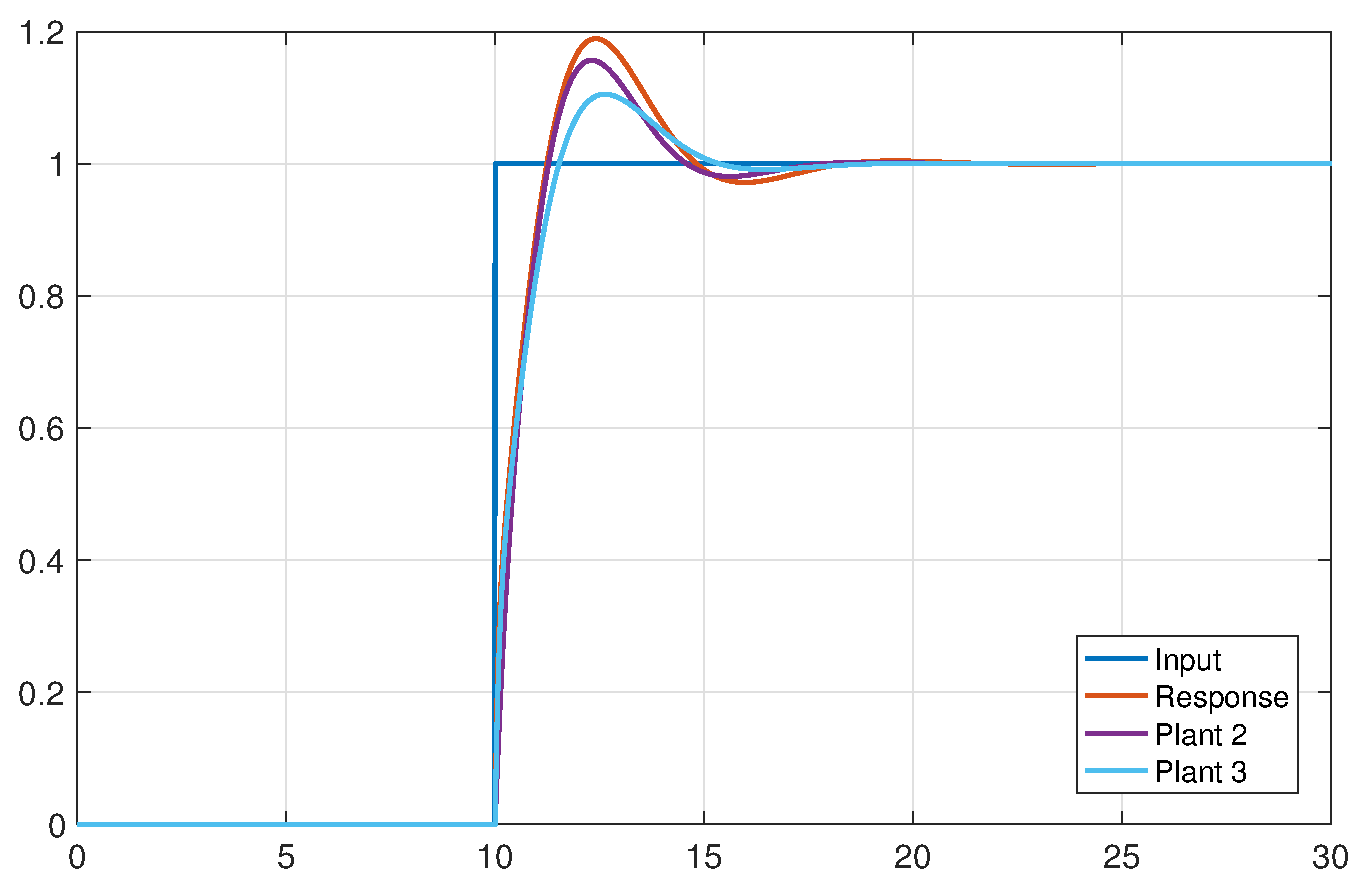
\includegraphics[trim = 0 0 0 0, clip, width=1\textwidth]{p2bres.eps}
 \vspace{-20pt}
 \caption{Expected Quanser Repsonse of PID Controller}
 \label{p2bres}
\end{minipage}
\hfill
\begin{minipage}{.495\textwidth}
\centering
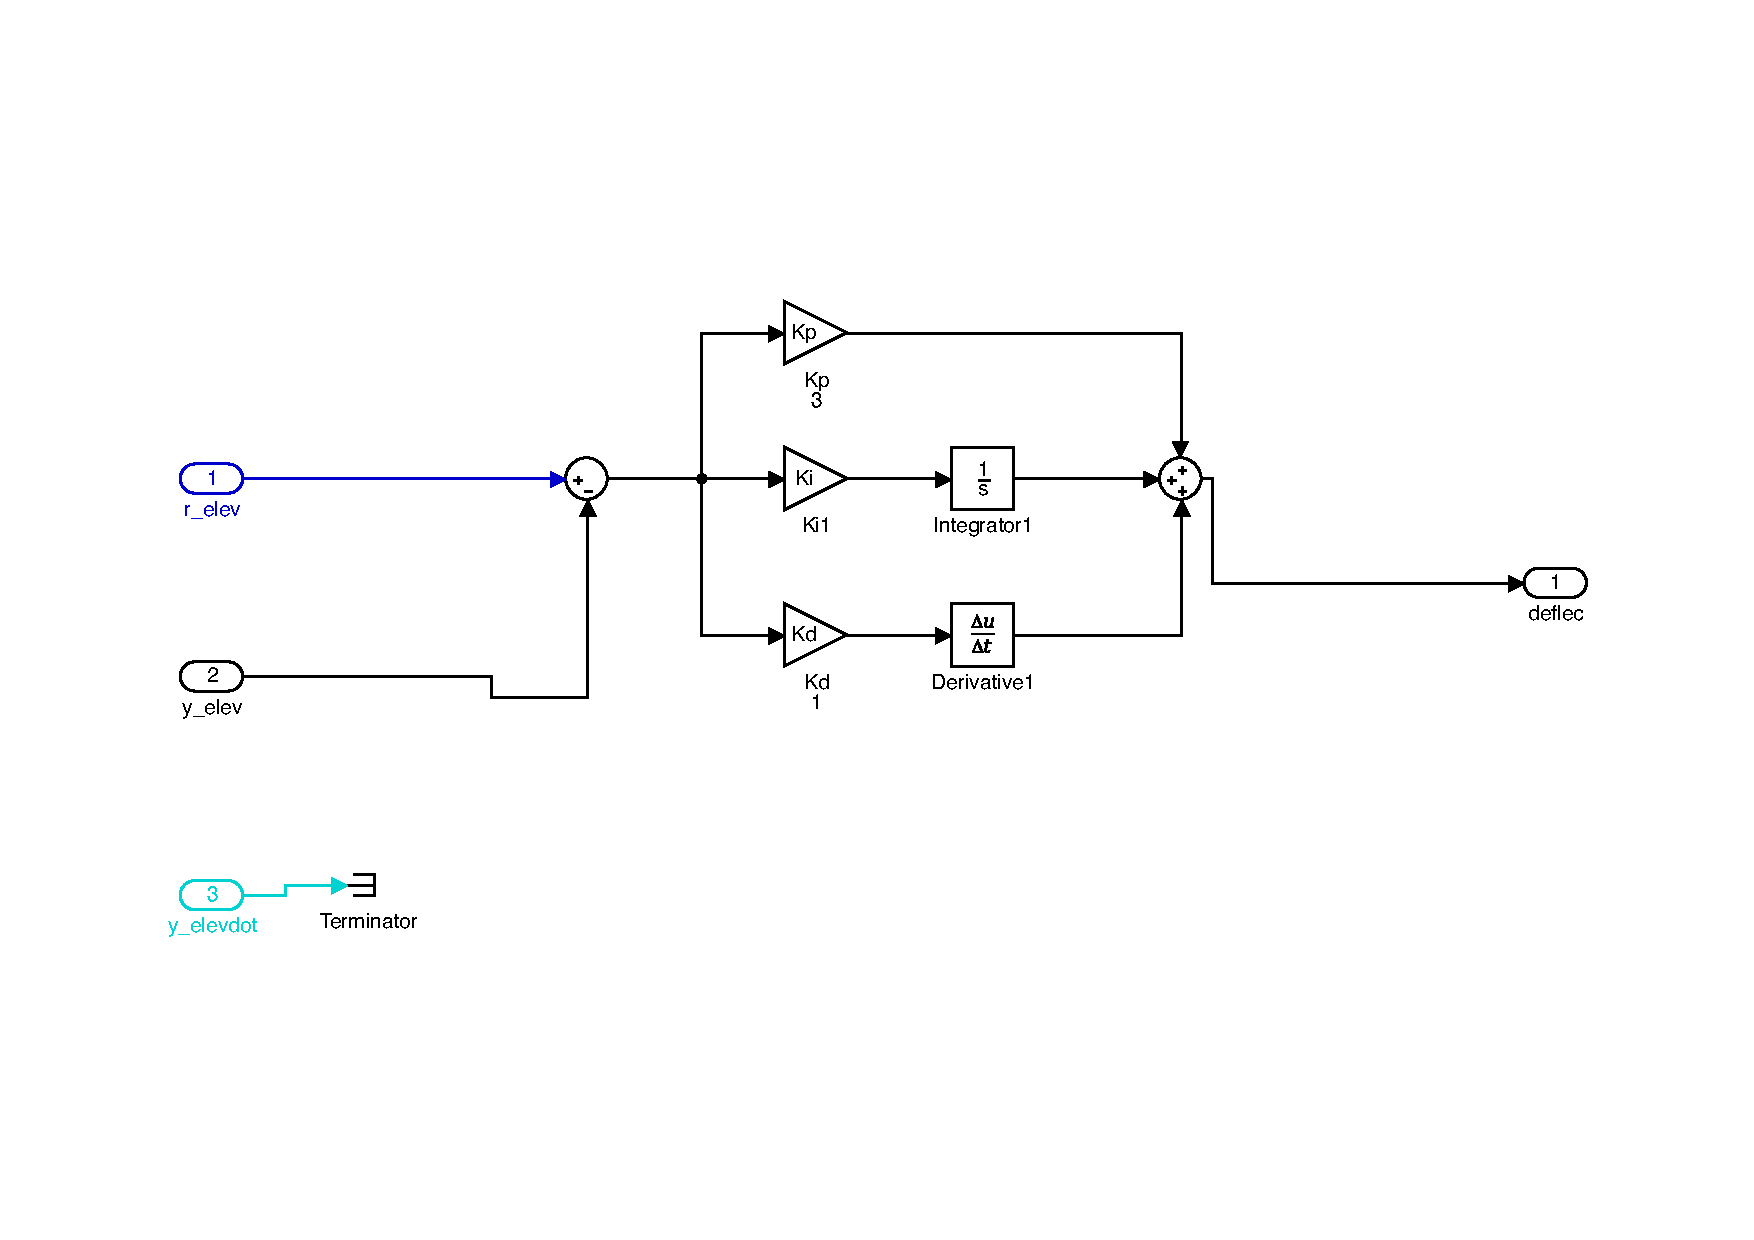
\includegraphics[trim = 0 0 0 0, clip, width=1\textwidth]{theorycontr.pdf}
\vspace{-10pt}
\caption{Simulation Used for Theory Controller}
\label{paramtab}
\end{minipage}
\vspace{-20pt}
\end{figure}
